\documentclass[11pt, oneside]{article}   	% use "amsart" instead of "article" for AMSLaTeX format
\usepackage{geometry}                		% See geometry.pdf to learn the layout options. There are lots.
\geometry{letterpaper}                   		% ... or a4paper or a5paper or ... 
%\geometry{landscape}                		% Activate for for rotated page geometry
%\usepackage[parfill]{parskip}    		% Activate to begin paragraphs with an empty line rather than an indent
\usepackage{graphicx}				% Use pdf, png, jpg, or eps� with pdflatex; use eps in DVI mode
								% TeX will automatically convert eps --> pdf in pdflatex		
\usepackage{amssymb}
\usepackage{amsmath}
\usepackage{parskip}
\usepackage{color}
\usepackage{hyperref}

\title{Cauchy's Formula}
%\author{The Author}
%\section{}
%\subsection*{}
\date{}							% Activate to display a given date or no date

\graphicspath{{/Users/telliott_admin/Dropbox/Tex/png/}}
% \begin{center} 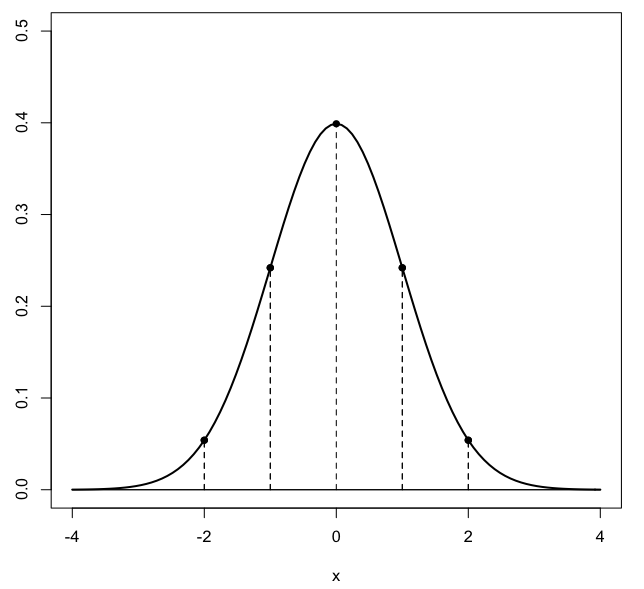
\includegraphics [scale=0.4] {gauss3.png} \end{center}
\begin{document}
\maketitle
\Large
\subsection*{Quick review}
We showed before that if $f(z)$ is analytic everywhere in a domain and we integrate around a closed path enclosing that region
\[ I = \oint f(z) \ dz = 0 \]
On the other hand, if the region includes a singularity, the value of the integral is independent of the path (but non-zero because of the singularity).

We obtain the same value for the line integral around any path.  If that path encloses a singularity, then the value of the integral is non-zero.

So consider any $z_0$ in the domain
\[ \oint \frac{f(z)}{(z-z_0)} \ dz \]
Parametrize $z$ as a circle of radius $\rho$ centered on $z_0$
\[ z = z_0 + \rho e^{i\theta} \]
\[ dz = i \rho e^{i\theta} \ d \theta \]
then 
\[ I =  \oint \frac{f(z)}{(z-z_0)} \ dz \]
\[ = \oint \frac{f(z_0 + \rho e^{i\theta})}{ \rho e^{i\theta}} \ i \ \rho e^{i\theta} \ d \theta \]
\[ = i \oint f(z_0 + \rho e^{i\theta}) \ d \theta \]
Since we have the same value for \emph{any} path, imagine that that $\rho \rightarrow 0$ so $z \rightarrow z_0$ and then in the limit we have
\[ I = i \oint f(z_0) \ d \theta \]
but $f(z_0)$ is a constant value so it can come out from the integral
\[ I = i  f(z_0) \oint \ d \theta = 2 \pi i \  f(z_0) \]
\[ \oint \frac{f(z)}{(z-z_0)} \ dz = 2 \pi i \  f(z_0) \]

\subsection*{example}
We can use the inverse function ($1/z$) as an example.  This function has a singularity at the origin.  Compare with the form of Cauchy2:
\[  \oint \frac{f(z)}{z - z_0} \ dz = 2 \pi i f(z_0) \]
We can match this form if we set $f(z) = 1$ and $z_0 = 0$.  The theorem says we can write the value of the integral as
\[ I = 2 \pi i f(z_0) = 2 \pi i \]
This matches what we obtained by parametrizing the unit circle.  There we had
\[ z = e^{i\theta}, \ \ \ \theta = 0 \rightarrow 2 \pi \]
\[ dz = iz \ d \theta \]
\[ \oint \frac{1}{z} \ dz = \int_0^{2\pi} i \ d \theta = 2 \pi i \]
This is $2 \pi i$ times the value of the function at $z_0 = 0$, which is $1$.

\subsection*{example}
Consider
\[ \oint \frac{6}{z(z-3)} \ dz \]
As shown in the figure, we are supposed to take for the curve $C$ the set of points $|z-3| = 5$, which is a circle of radius $5$ surrounding the point $z=3+0i$.
\begin{center} 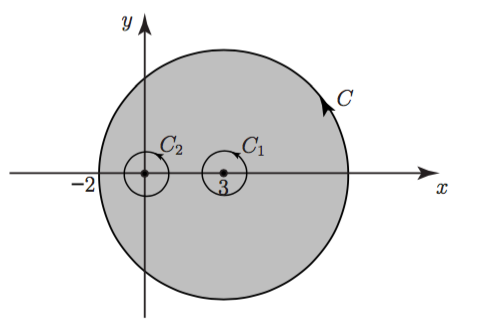
\includegraphics [scale=0.5] {cauchy2-fig1.png} \end{center}
This function does have two points of singularity, namely $z=0$ and $z=3$, so we expect that the value of the integral will not be zero.  We use (4) above to write
\[ \oint_C f(z) \ dz = \oint_{C_1} f(z) \ dz + \oint_{C_2} f(z) \ dz \]
We do not need to specify the curves because we will use (3) to calculate the values.

However, we do need to manipulate the function a bit.  We use the method of partial fractions.  Leaving aside the factor of $6$ for a moment:
\[ \frac{1}{z(z-3)} = \frac{A}{z} + \frac{B}{z-3} = \frac{A(z-3) + B(z)}{z(z-3)} \]
From looking at the numerator on the left- and right-hand sides, we see that $A = -B$ (because $Az + Bz = 0$), and that $-3A = 1$.  Hence
\[ A = -\frac{1}{3}, \ \ \ B = \frac{1}{3} \]
Recall the factor of $6$ and substitute for $A$ and $B$ in the middle expression to obtain:
\[ f(z) = \frac{-2}{z} + \frac{2}{z-3} \]
So now we can split the integrals for each curve into two parts.  We have:
\[ I = \oint_{C_1} f(z) \ dz + \oint_{C_2} f(z) \ dz \]
\[ = \oint_{C_1} \frac{-2}{z} \ dz + \oint_{C_1} \frac{2}{z-3} \ dz + \oint_{C_2} \frac{-2}{z} \ dz + \oint_{C_2} \frac{2}{z-3} \ dz  \]
Two of these four parts do not contain poles (the first and last), so those are just zero, and we have
\[ I = \oint_{C_1} \frac{2}{z-3} \ dz + \oint_{C_2} \frac{-2}{z} \ dz  \]
At this point we can use (3) from above, that
\[ \oint_C \frac{f(z)}{z - z_0} \ dz = 2 \pi i f(z_0) \]
(recognizing that the denominator for the second integral can be written as $z - 0$).  So the result is $2 \pi i f(z_0)$ for both integrals, but the value of the function is just $2$ for the first term and $-2$ for the second term, which cancel.  In this case, the total integral is just zero.
Notice that the cancellation comes because $A = -B$, which we would obtain for any two factors $z$ and $z - a$ ($a \ne 0$), as long as the function itself is a constant
\subsection*{example}
Consider
\[ \oint \frac{z}{z^2 + 1} \ dz \]
This function has poles at $z = \pm i$.
\begin{center} 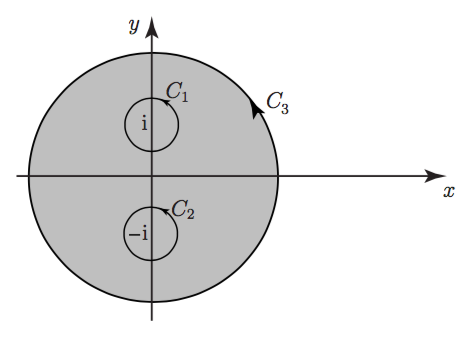
\includegraphics [scale=0.5] {cauchy2-fig2.png} \end{center}
We could find where the poles are by solving $z^2 + 1 = 0$ or we could factor
\[ z^2 + 1 = (z + i)(z - i) \]
This leads us to the strategy of partial fractions as before
\[ \frac{z}{z^2 + 1} = \frac{A}{z+i} + \frac{B}{z-i} \]
By inspection, $A = B = 1/2$ is a solution, so
\[ \oint \frac{z}{z^2 + 1} \ dz = \oint \frac{1/2}{(z+i)} + \frac{1/2}{(z-i)} \ dz  \]
As before, curve $C_1$ encloses a pole only for the second term, and $C_2$ for the first term.  We use
\[ \oint_C \frac{f(z)}{z - z_0} \ dz = 2 \pi i f(z_0) \]
where the function is simply the value $1/2$ at both points.  So we obtain
\[ 2 \pi i \  \frac{1}{2} = \pi i \]
for \emph{each} pole.

Another way is to write
\[ \frac{z}{z^2 + 1} = \frac{z}{(z + i)(z - i)} = \frac{z/z+i}{z-i} \]
For $C_1$, this has a pole at $z=i$, so the value of the integral is
\[ 2 \pi i \ f(z_0) = 2 \pi i \ \frac{i}{i+i} = \pi i \]
For $C_2$
\[  \frac{z/z-i}{z+i} \]
At the pole $z=-i$, the value of $f(z) = z/z-i$ is again $1/2$.

Yet another way to obtain this result, by analogy to calculus of real variables.  Substitute
\[ w = z^2 + 1 \]
\[ dw = 2 z \ dz \]
\[ \oint \frac{z}{z^2 + 1} \ dz = \frac{1}{2} \int \frac{1}{w} \ dw \]
\[ = \frac{1}{2} \ \text{Log} \ (w)   \]
\[ =  \frac{1}{2} \ \text{Log} \ (z^2 + 1)   \]
\[ \text{Log} \ z^2 = \text{Log} \ r^2 e^{i2\theta} = \ln r + 2 i \theta \]
if we evaluate over a closed contour ($\theta = 0 \rightarrow 2 \pi$) the terms with $\ln r$ vanish and we have then $4 \pi i$ times one-half or $2 \pi i$.
(Problem with the sum $+1$?

\subsection*{example}
\[ I = \int \frac{z^2}{4-z^2} \ dz \]
on the circle of radius $2$ centered at $z_0 = -1 + 0i$
\[ \gamma(\theta) = z_0 + 2e^{i \theta} = 1 + 2e^{i \theta} \]
Notice that the zeroes of the denominator occur at $z = \pm \ 2$ and that one of these is contained within our path of integration.

If we factor the denominator
\[ \frac{1}{4-z^2} = \frac{1}{4} \ [ \ \frac{1}{2-z} + \frac{1}{2+z} \ ] \]
we can split the integral
\[ I = \frac{1}{4} \int \frac{z^2}{2-z} + \frac{z^2}{2+z} \ dz \]
The first one is just zero, by Cauchy's theorem.  The second term contains the singularity:
\[ I = \frac{1}{4} \int \frac{z^2}{2+z} \ dz \]
Here $f(z) = z^2$ and 
\[ z - z_0 = z + 2 \]
so $z_0 = -2$ so the value of the manipulated integral is
\[ 2 \pi i \ f(z_0) = 2 \pi i \ 4 = 8 \pi i \]
and the value of the original one is
\[ I = \frac{1}{4} 8 \pi i = 2 \pi i \]


\end{document} 